% Section: Introduction

With an increasing amount of electronically distributed unstructured text
(newspapers, letters etc.) there is a growing demand for its analysis and
understanding by computer means. This process should be as automated as possible
due to the time consumption and huge data amount.

\textan{} (Text Analyser) serves this purpose. In other words, \textan{} is a
tool that processes structured data buried in plain text documents and provides
basic operations to manipulate the extracted data. The extraction consists of
recognizing significant phrases, matching them with data already stored in the
database and discovering dependencies expressed in the text. The first two tasks
are semi-automatic in \textan{}, whereas the last one is manual only. The
objective of \textan{} is to provide a robust tool which supports the procedure.
Although first impulse came from the Police needs, \textan{} is made as general as
possible to allow easy configuration for any other domain as needed.

\section{System overview}
The system consists of two main components -- the client application
and the server. For information intended for end-users about client usage, see
Section \ref{sec:ClientUsage}. Instruction intended for system
administrators can be found in Chapter \ref{sec:AdminGuide}, mainly in Section
\ref{sec:Client} about configuring the client and in Section \ref{sec:Server}
about server configuration.

Users of \textan{} can manage the stored documents. The unprocessed documents
can be inserted into the system for later use. Full text search supports both
unprocessed and processed documents and more sophisticated search methods can be
performed on annotated reports. Users can annotate unprocessed documents stored
in the database or completely new reports either imported from local files or
written from scratch. See Figure \ref{fig:Overview} for simplified document
lifecycle diagram.

\begin{figure}[!htb]
        \centering
        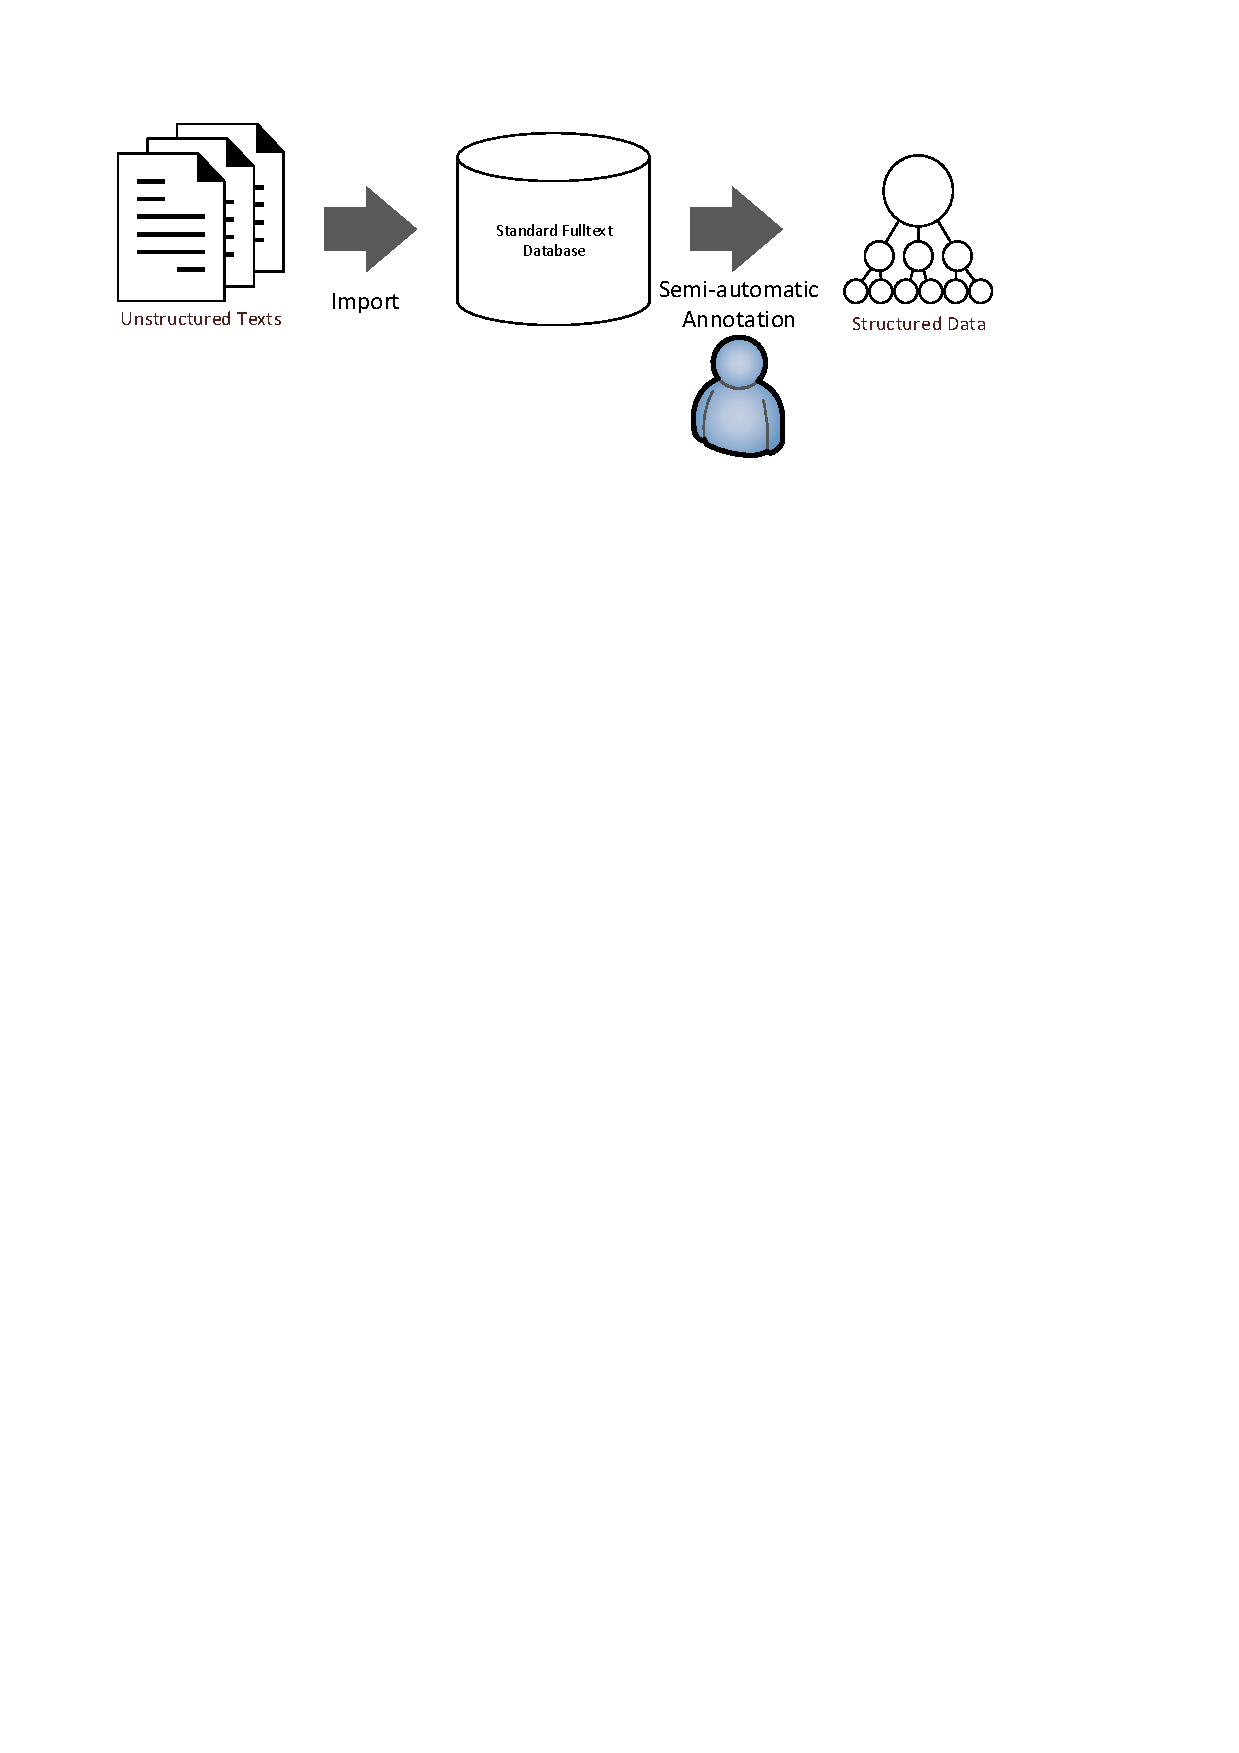
\includegraphics[width=\textwidth]{Images/Overview}
        \caption{Simplified document lifecycle.}
        \label{fig:Overview}
\end{figure}

This documentation describes \textan{} from the user and administrator
perspective.

\section{Glossary}
Terms are used in very specific manner in the documentation and in both the
client and the server, therefore it is really essential to understand their
meaning. Otherwise, it is possible to misunderstand the rest of the text.

\comment[anyone]{Petr}{check if this makes sense!}
\begin{description}
\item[Document]
The document is an arbitrary text that is processed by \textan{}. E.g. a police
report, a letter, a movie review or a judgment. In the following text the terms
document and report are used interchangeably.

\item[Object]
The term "object" refers to our representation of some unique thing in
\textan{}. Consider for example a person with name Joseph Smith from Prague with
identifier 000123/4567. The object refers to this person in the real world, in
meat and bones.

\item[Alias]
The alias represents a designation of a object. For example: Joseph Smith, Joe
Smith, Joey S., J. Smith or just Smith can be names of one concrete person.
Names are aliases for the person.

\item[Entity]
An entity is a sequence of words recognized either by a named entity recognizer
or by a user. \comment[Petr]{Petr}{Move to next paragraph - Object assigment}
The entity will be later assigned to an object and it becomes an alias
of the object. Consider for example the sentence: Joe Smith was seen
in Prague on 5th September. The sentence contains 3 entities: Joe Smith (person),
Prague (city), 5th September (date). We don't know which objects belong to these
entities yet. Prague can represent the capital city of the Czech Republic,
or a city in the USA.

\item[Object/Entity Type]
Each object and each entity has a type. For example person, date, city, country
etc. The set of types in the system depends on the domain which the system is
deployed to.

\item[Object Assigment]
\comment[Petr]{Petr}{Description of object assigment}

\item[Alias occurrence]
\comment[Petr]{Petr}{Description of alias occurence}

\item[Object Merging]
\comment[Petr]{Petr}{Description of object merging}

\item[Relation]
The relation represents any relationship between objects mentioned in a document.
A relation can be represented in a document by an anchor word, or it can be
unexpressed, which means without any anchor in a document. See Anchor below.
\comment[anyone]{Adam}{Check this sentence with two relations, one with anchor, one without anchor.}
Consider this example: "Adam (890524/1367) is married to Eve". Three objects
appear in the sentence - persons Adam and Eve and the id 890524/1367. There
are two relations: Adam "has" 890524/1367 without an anchor and Adam "marriage"
Eve with the anchor "married".

\item[Relation Type]
Each relation has a type. For example born, reside, die, kill etc. Similarly to
object/relation types the set of relation types in the system depends on the
domain which the system is deployed to.

\item[Anchor]
An anchor is a word or a sequence of words that is bound to a relation between
objects. Consider for example the sentence: Joey Smith killed Mary-Ann S. There
is a relation between Joey Smith and Mary-Ann S., which is represented by the
word "killed". The word is the anchor. \comment{Ondrej}{Why do you not write
about type here?}

\item[Roles and orders]
Each object in a relation can have a role assigned. This role is mostly used
for visualisation and storing additional information. Moreover object can also
have order assigned which is just an integral number used for graph
visualization\ifdefined\USRDOC{} (see Section \ref{sssec:EditRelations})\fi{}
\ifdefined\DEVDOC{} (see Section \ref{USR-sssec:EditRelations} in the user
documentation)\fi{}. For example relation created from sentence
"Bill killed Joe." could be represented like this:
Bill (-1, murderer) --kill--> (1, victim) Joe.
\end{description}


